In the previous section have been analyzed the goals of Stratum V2, especially in regards to the inefficiencies related to its predecessor. \\
Before entering into the detailed differences between SV1 and SV2, it's necessary to provide a concise explanation about the new \textbf{sub-protocols}, \textbf{roles}, and \textbf{channel types}, introduced and standardized by the Stratum V2 protocol specifications.\\
\subsubsection{Roles}
The roles involved in data flow can be classified as either downstream or upstream in relation to each other. Here are the roles and their respective classifications:
\begin{itemize}
    \item \textbf{Mining Device} \\ The mining device is the physical hardware that carries out the hashing process.
    It is considered the most downstream role.

    \item \textbf{Pool Service} \\ This role belongs to the entity where the actual hashrate produced by the mining devices is consumed. It is considered the most upstream role.

    \item \textbf{Mining Proxy} \\ This role represents the proxy server situated between the mining device and the pool service. It handles message coordination and aggregation. In relation to the mining device, it is considered upstream, while in relation to the pool service, it is considered downstream.

    \item \textbf{Job Negotiator} \\ The job negotiator receives transactions from the Template Provider (which is essentially the Bitcoin client) and constructs custom block templates. It also negotiates the use of these templates with the pool. 

    \item \textbf{Template Provider} \\ This role is fulfilled by a Bitcoin client responsible for generating custom block templates. These templates are then sent to the Job Negotiator for mining purposes.\\
\end{itemize}

\subsubsection{Sub-protocols}
To fulfill the goals related to pooled mining operations efficiency, decentralization of the transaction selection process, and the other aspects previously declared, Stratum V2 had to introduce some new sub-protocols. Regarding the main mining protocol, new types of communication channels were standardized.

\begin{itemize}
    \item \textbf{Mining Protocol} \\The mining protocol is the primary protocol used for mining and serves as the direct successor to Stratum (V1). It enables communication between a mining device and its upstream node, pool, or proxy. This protocol is essential and must be implemented in all mining scenarios. In cases where a miner or pool does not support transaction selection, the mining protocol is the only protocol used.\\
    The protocol defines three types of communication channels:
    \begin{itemize}\label{channels}
        \item \textbf{Standard channels}\label{sssec:sv2_hom}: they don't manipulate the Merkle path / coinbase transaction, greatly simplifying the communication required between them and upstream nodes.
        \item \textbf{Extended channels}: they are given extensive control over the search space so that they can implement advanced use cases (e.g. translation between V1 and V2, difficulty aggregation, custom search space splitting, etc.).
        \item \textbf{Group channels}: they are simply collections of standard channels that are opened within a particular connection so that they are addressable through a common communication channel.
    \end{itemize}
    
    \item \textbf{Job Negotiation Protocol} \\ The job negotiation protocol is utilized by a miner, typically a mining farm, to negotiate a block template with a pool. The results of this negotiation can be reused for all mining connections to the pool, reducing computational intensity. In other words, a single negotiation can be applied to an entire mining farm or even multiple farms with a large number of devices, leading to greater efficiency. This protocol is separate to allow pools to terminate these connections on separate infrastructure from mining protocol connections.
    \item \textbf{Template Distribution Protocol} \\ The template distribution protocol shares a similar structure to facilitate obtaining information about the next block from Bitcoin Core. It is designed to replace \textit{getblocktemplate} with a more efficient and easier-to-implement solution for those incorporating other aspects of Stratum V2 into their systems.
\end{itemize}

\begin{figure}[h!]
    \centering
    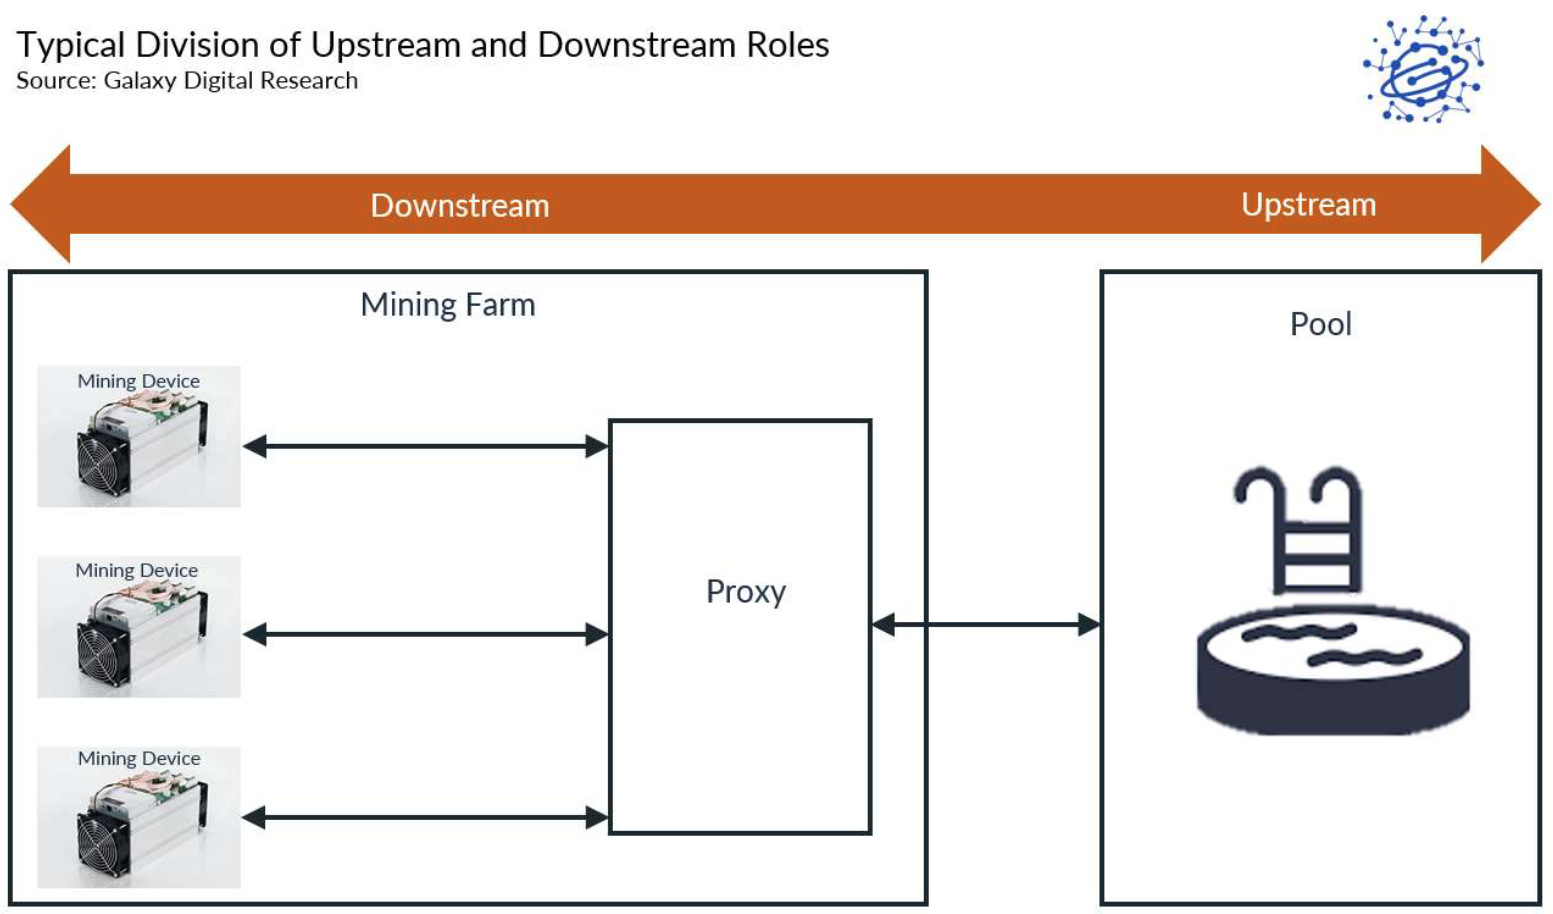
\includegraphics[width=15cm]{Figures/sv2/sv2_2.png}
    \caption{Typical Division of Downstream and Upstream Roles, \textit{Galaxy Digital Research} \cite{galaxyFutureBitcoin}}
    \label{fig:sv2_2}
\end{figure}

To better understand the list of differences between SV1 and SV2 which will follow, a preface with some more deep aspects which regard the SV2 protocol choices in term of protocol security, binary framing, and censorship resistance enhancements is needed.

\subsubsection{SV2 protocol security}\label{sssec:sv2:security} <<Stratum V2 employs a type of encryption scheme called AEAD (authenticated encryption with associated data) to address the security aspects of all communication that occurs between clients and servers. This provides both confidentiality and integrity for the ciphertexts (i.e. encrypted data) being transferred, as well as providing integrity for associated data which is not encrypted. Prior to opening any Stratum V2 channels for mining, clients MUST first initiate the cryptographic session state that is used to encrypt all messages sent between themselves and servers. Thus, the cryptographic session state is independent of V2 messaging conventions.\\
At the same time, the SV2 protocol specification proposes optional use of a particular handshake protocol based on the Noise Protocol framework \cite{noiseprotocolNoiseProtocol}. The client and server establish secure communication using Diffie-Hellman (DH) key agreement, as described in greater detail in the Authenticated Key Agreement Handshake section of the specifications document.\\
Using the handshake protocol to establish secured communication is optional on the local network (e.g. local mining devices talking to a local mining proxy). However, it is mandatory for remote access to the upstream nodes, whether they be pool mining services, job negotiating services or template distributors.>> \cite{githubSv2spec04ProtocolSecuritymdMain}\\\\

\subsubsection{SV2 binary framing}\label{sssec:sv2_framing}
The Stratum V2 protocol is binary, with fixed message framing. Each message begins with the extension type, message type, and message length (six bytes in total), followed by a variable length message. Figure \ref{fig:sv2_4} describes the message framing used by the protocol.

\begin{figure}[h!]
    \centering
    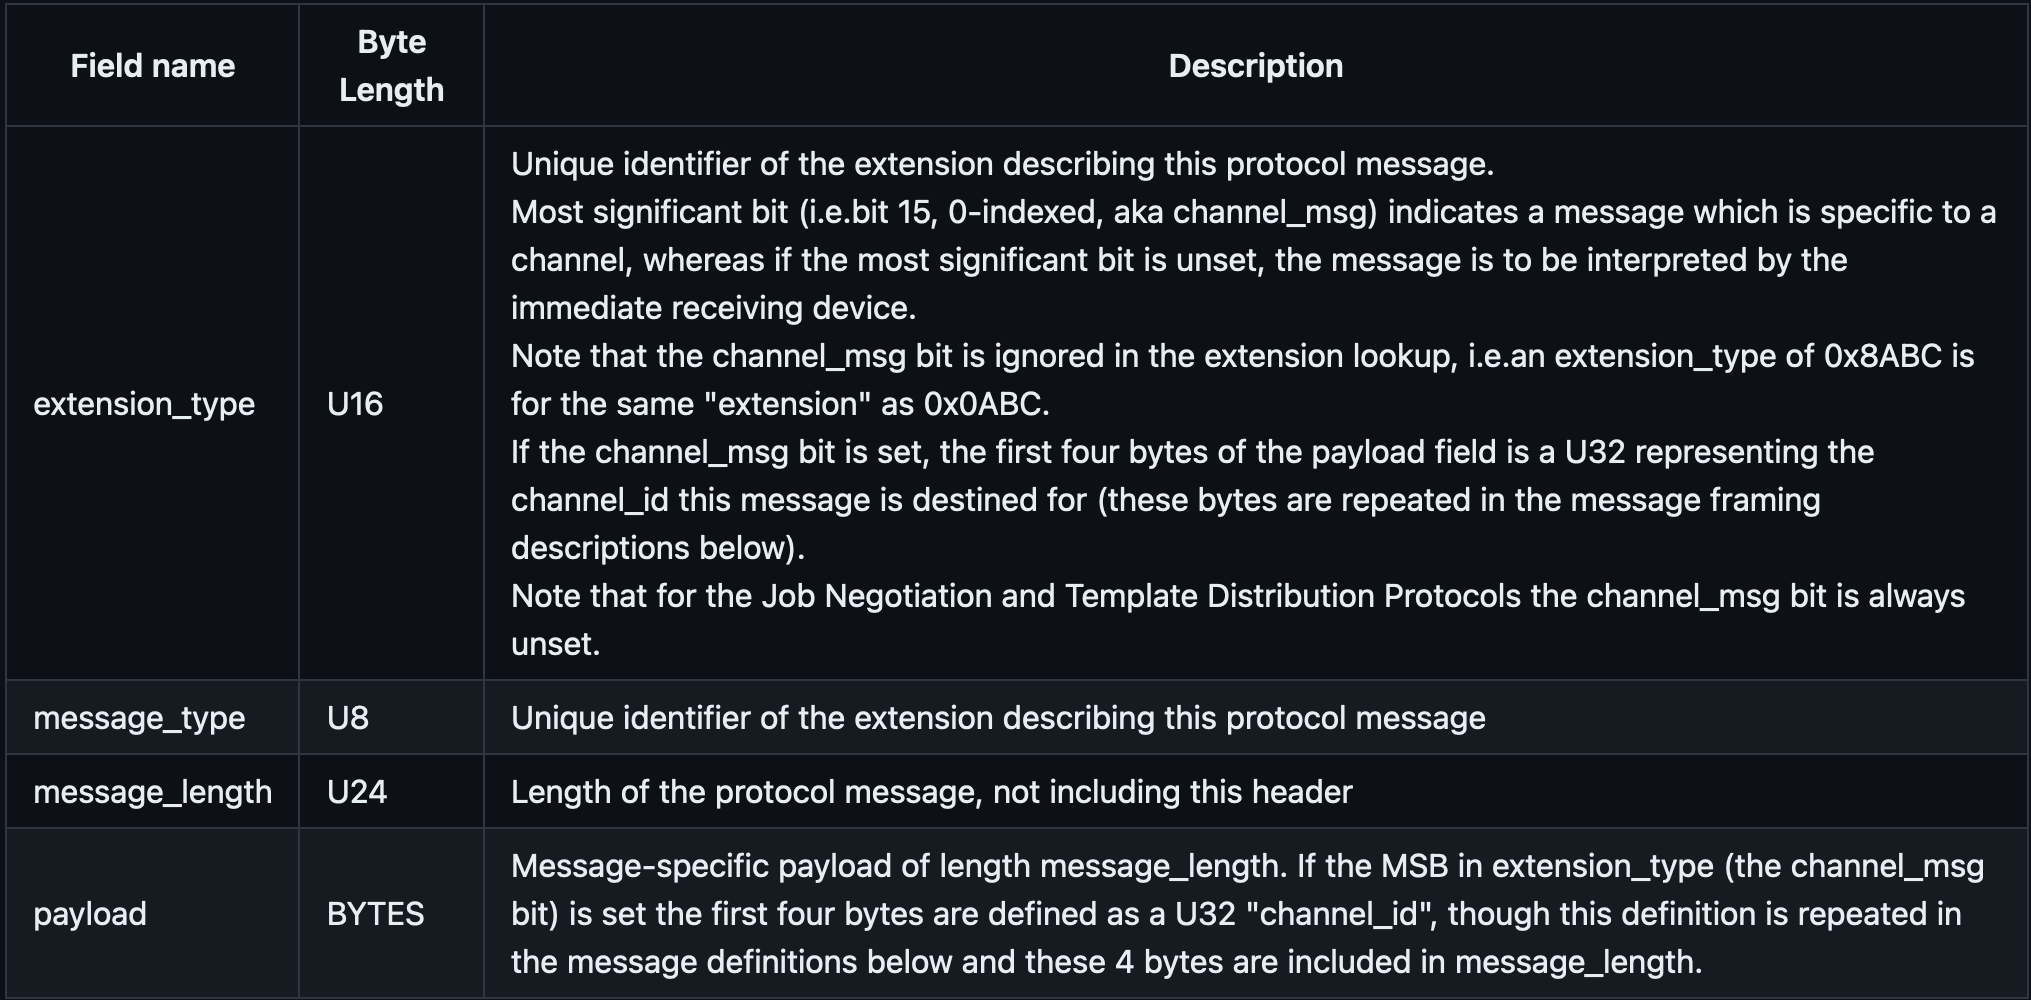
\includegraphics[width=15cm]{Figures/sv2/sv2_4.png}
    \caption{SV2 protocol binary framing}
    \label{fig:sv2_4}
\end{figure}

\subsubsection{SV2 transaction selection}
In section \ref{section:stratum}, related to Stratum (V1), it's well explained how the current pooled mining operations work.
Today, the selection of the transactions to be inserted in the block templates, which are distributed in the form of jobs to the miners, is a pool responsibility. The only entities who took valid Bitcoin transactions from the mempool and decide the ones who will be mined in the next block are the pool operators. Since pool are public entities, they can be attacked from governments, and this is not so ideal for the censorship-resistance property of the Bitcoin network as a whole. \\ 
With Stratum V2, miners now have the ability to choose their own work (i.e. choose their own transaction set), making mining process more decentralized. This is implemented separately from the main mining protocol, as described previously, and it is optional for pools and miners. In Figure \ref{fig:sv2_3}, it's very clear the benefits that will be brought by having miners (single miners, mining farms, etc.) selecting transactions from their local bitcoin node's mempool, and negotiating their own block template with the pool, instead relaying on the pool responsibility.\\

\begin{figure}[h!]
    \centering
    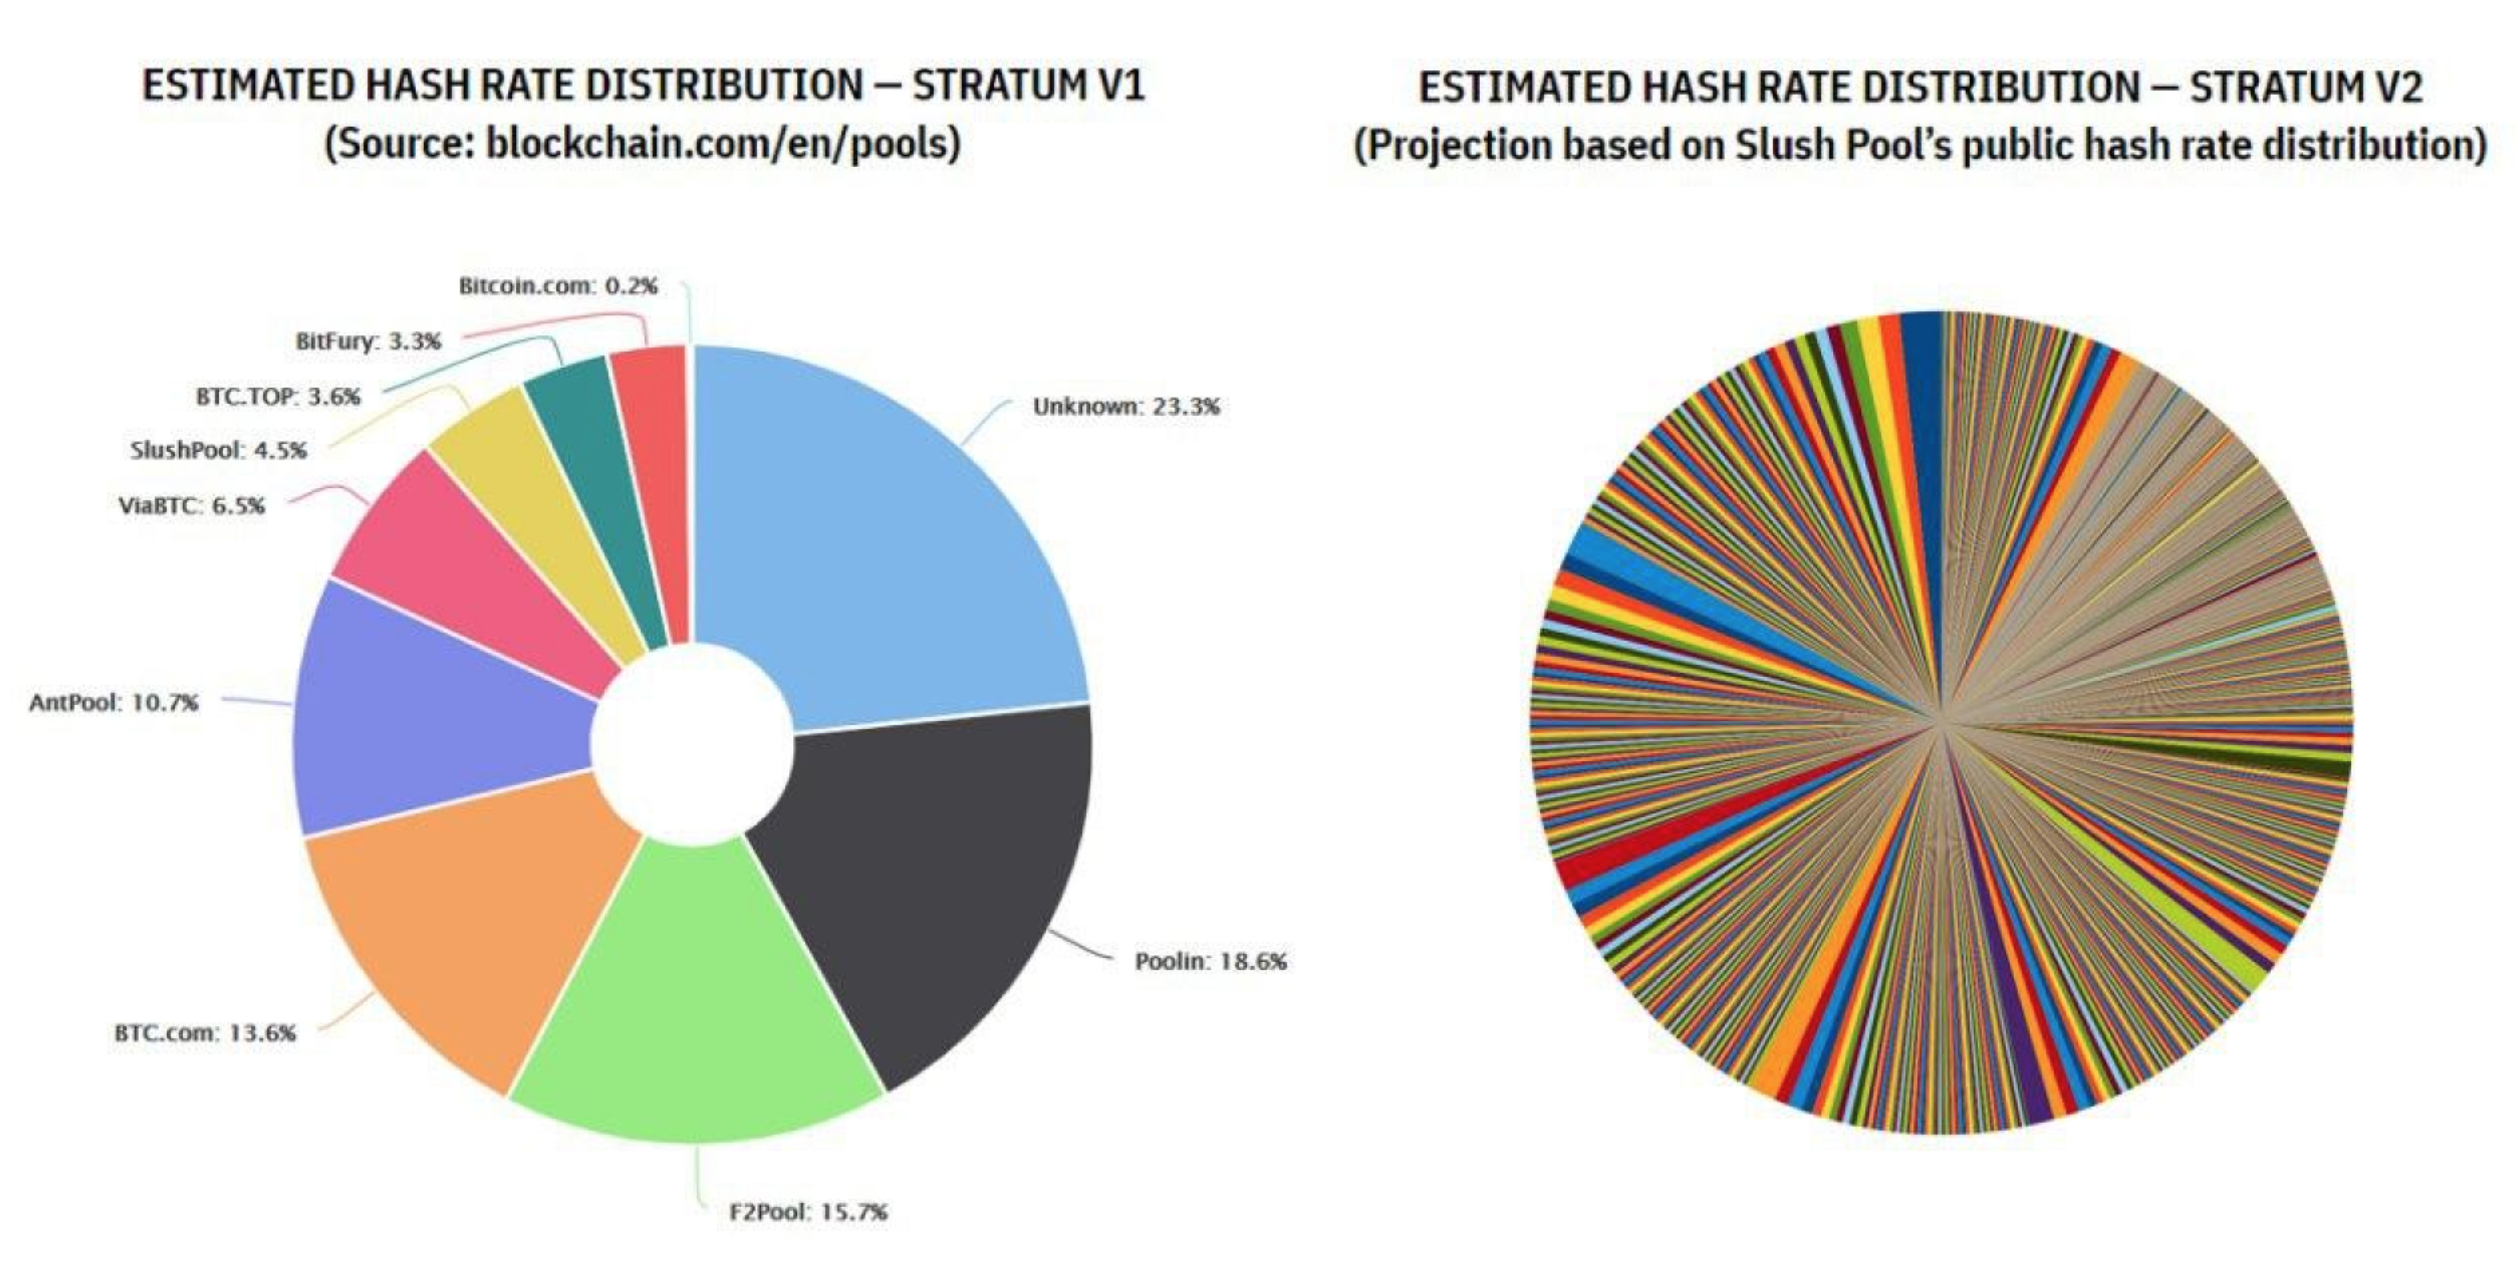
\includegraphics[width=15cm]{Figures/sv2/sv2_3.png}
    \caption{Transaction selection decentralization brought by Stratum V2 \cite{braiinsBitcoinsDecentralization}}
    \label{fig:sv2_3}
\end{figure}